%%%%%%%%%%%%%%%%%%%%%%%%%%%%%%%%%%%%%%%%%%%%%%%%%%%%%%%%%%%%%%%%%%%%%%%
% file
% bismon/talks/Lamsade-21nov2019/Bismon-Starynkevitch-Lamsade-21nov2019.tex
% in http://github.com/bstarynk/bismon/
% inspired by http://cse.unl.edu/~cbourke/latex/UNLTheme.tex
%%%%%%%%%%%%%%%%%%%%%%%%%%%%%%%%%%%%%%%%%%%%%%%%%%%%%%%%%%%%%%%%%%%%%%%

\documentclass[xcolor=svgnames,final,smaller,a4]{beamer}
\usepackage{relsize}
\usepackage{luacode}
\usepackage{xcolor}
\usepackage{alltt}
\usepackage{listings}
\usepackage{hyperref}


\hypersetup{
  colorlinks   = true, %Colours links instead of ugly boxes
  urlcolor     = NavyBlue, %Colour for external hyperlinks
  linkcolor    = DarkGreen, %Colour of internal links
  citecolor   = DarkMagenta, %Colour of citations
  frenchlinks = true,
}

\usetheme[hideothersubsections]{Bismon}



\title{\textsc{Bismon} \\
a static source code analysis framework using \textit{some} symbolic artificial intelligence techniques.}
\author[B.Starynkevitch]{Basile \textsc{Starynkevitch} - \href{http://starynkevitch.net/Basile/}{\texttt{starynkevitch.net/Basile}}\\
  \href{mailto:basile.starynkevitch@cea.fr}{\color{blue}{\texttt{basile.starynkevitch@cea.fr}}} and \href{mailto:basile@starynkevitch.net}{\color{blue}{\texttt{basile@starynkevitch.net}}}
} %
\institute{ \raisebox{0.4cm}{CEA/LIST (DILS) - laboratoire de Sûreté des Logiciels -} 
\includegraphics[scale=0.14]{CEA-LIST-logo}}
\date{November 21\textsuperscript{st}, 2019}

\begin{document}
 \begin{luacode*}
   local gitpip=io.popen("git log --no-color --format=oneline -1 --abbrev=16 --abbrev-commit -q | cut -d' ' -f1")
   gitid=gitpip:read()
   gitpip:close()
 \end{luacode*}
 \newcommand{\mygitid}{\luadirect{tex.print(gitid)}}
 \newcommand{\Bismon}{\href{https://github.com/bstarynk/bismon}{\textsc{Bismon}}}

%{% open a Local TeX Group
%\setbeamertemplate{sidebar}{}
 \begin{frame}
   
   
   \begin{relsize}{-1.5}
        \titlepage
        \textcolor{brown}{{\large \textbf{Opinions are only mines}} (not from  CEA or E.C.)}
        
        \begin{center}
         

          git \texttt{\mygitid}
        \end{center}
   \end{relsize}
\end{frame}
%}% end Local TeX Group


\section{Introduction}

\begin{frame}
    \frametitle{Introduction}
    \framesubtitle{funding}

    {\Bismon} is funded by two \href{https://ec.europa.eu/programmes/horizon2020/en}{Horizon 2020} research and innnovation actions:
    
    \begin{itemize}
    \item \href{https://www.chariotproject.eu/}{\textsc{Chariot}}, under Grant Agreement 780075.
      \item \href{http://decoder-project.eu/}{\textsc{Decoder}}, under Grant Agreement 824231.
    \end{itemize}

    So  {\Bismon} is European.

    \begin{center}
      
\includegraphics[width=0.15\textwidth]{Flag-of-Europe} \raisebox{0.4cm}[1pt][1pt]{(100\% funded by the European Commission)}.
    \end{center}
    
\end{frame}
    
\begin{frame}
    \frametitle{Introduction}
    \framesubtitle{AI and other inspirations}

    \begin{itemize}

    \item D.Lenat work on \textsc{Rll -1} then \textsc{Eurisko}
    \item J.Pitrat (1934 - 2019) pionneering work on \textsc{Caia}
    \item my PhD work (1985 - 1990)
    \item my past \href{http://starynkevitch.net/Basile/gcc-melt/}{\textsc{Gcc Melt}} work (2008 - 2016)
    \item \href{http://frama-c.com/}{\textsc{Frama-C}} and \textit{non-relational} databases
    \item \href{http://gcc.gnu.org/}{\textsc{Gcc}}  $> 10$MLOC of \textit{C++} {\relsize{-1}{(bootstrapped with \texttt{g++ -O2 -flto})}}
 and a dozen of \href{https://en.wikipedia.org/wiki/Domain-specific_language}{DSL}s
    \end{itemize}

    For references, see the \href{http://starynkevitch.net/Basile/bismon-chariot-doc.pdf}{{\Bismon} \textbf{draft} report} {\relsize{-1}{on my home page}}

    Some GPLv3+ code for \textsc{Linux/x86-64} desktop is available
    \href{http://github.com/bstarynk/bismon}{\texttt{github.com/bstarynk/bismon}}

    \hrule
    
    These slides are under \href{https://creativecommons.org/licenses/by-sa/4.0/}{
\includegraphics[scale=0.75]{CC-BY-SA-4}} \relsize{-1}{(CC-BY-SA-4)} and available from \href{http://starynkevitch.net/Basile/Bismon-Starynkevitch-Lamsade-21nov2019.pdf}{\texttt{starynkevitch.net/Basile/Bismon-Starynkevitch-Lamsade-21nov2019.pdf}}

    
    
\end{frame}

\begin{frame}
    \frametitle{Introduction}
    \framesubtitle{motivations}

    \textbf{Help} small teams of mostly \emph{junior} software developers (e.g. IoT) using \textsc{Linux} thru a collaborative \textit{Web} \emph{assistant} tool

    \begin{center}
      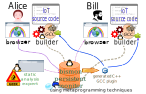
\includegraphics[width=0.90\textwidth]{bismon-monitor}
    \end{center}
    
\end{frame}
%%%%%%%%%%%%%%%%%%%%%%%%%%%%%%%%%%%%%%%%%%%%%%%%%%%%%%%%%%%%%%%%


\section{Data and persistence}

\begin{frame}
    \frametitle{Data and persistence}
    \framesubtitle{the \emph{Bismon} heap \textbf{\large greatly simplified}}

    \begin{center}
      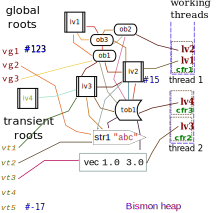
\includegraphics[width=0.72\textwidth]{heap-bismon}
    \end{center}
\end{frame}

\end{document}
%%%%%%%%%%%%%%%%%%%%%%%%%%%%%%%%%%%%%%%%%%%%%%%%%%%%%%%%%%%%%%%%
%% Local Variables: ;;
%% compile-command: "./build.sh" ;;
%% End: ;;
%%%%%%%%%%%%%%%%%%%%%%%%%%%%%%%%%%%%%%%%%%%%%%%%%%%%%%%%%%%%%%%%
